%
%

Absolute stellar ages are some of the most sought after astrophysical quantities. This is particularly true for identifiably young systems, where absolute ages provide our only constraints on time-dependent features of star and planet formation and evolution. Examples include placing constraints on the lifetime of primordial gas disks \citep[e.g.,][]{Haisch2001, Mamajek2009}, the timescale for giant planet formation \citep{Chabrier2014}, the giant planet migration timescale \citep{}, star formation timescales \citep{Pecaut2016}, and deriving the sub-stellar initial mass function \citep{Chabrier2003}. Unfortunatey, accurate absolute ages for young stars remain elusive \citep{Soderblom2014} due largely to a necessary reliance on stellar evolution models, which are beset with problems at ages younger than 100 Myr \citep[e.g.,][]{Mathieu2007, Stassun2014}. {\bf This proposal aims to develop stellar models and supporting theoretical tools necessary to establish accurate and precise ages for young stars.}

The textbook picture of early stellar evolution involves the quasi-hydrostatic collapse of a homogeneous gas sphere from an arbitrarily large initial radius down to a star where core hydrogen burning maintains hydrostatic equilibrium \citep[e.g.,][]{Henyey1955, Hayashi1961, Iben1965}. The four standard equations of stellar structure (mass conservation, hydrostatic equilibrium, energy conservation, energy transport) are assumed to be sufficient to describe the protostar's evolution \citep{Iben1965, Bodenheimer1965}. However, 
%``standard'' stellar evolution models constructed within this paradigm appear to provide an incomplete description of early stellar evolution. 
empirical Hertzsprung-Russell diagrams (HRDs) for young stellar populations exhibit a number of features that challenge this simple evolutionary picture \citep{Naylor2009, DaRio2010a, Herczeg2015}. 

Figure~\ref{fig:badhrd} illustrates two problems with ``standard'' stellar evolution models constructed within this simple theoretical paradigm. First, the observational data (grey points) exhibit a significant spread in luminosity at a given effective temperature, whereas standard models predict a tight sequence (black lines). Luminosity spreads such as the one shown in Figure~\ref{fig:badhrd} are a common feature among stellar populations with suspected ages $\lesssim 20$~Myr \citep{Hillenbrand1997, Hartmann2001, DaRio2010a}. A perfectly tight sequence such as that predicted by standard models is not expected, there will be some intrinsic width due to observational errors. However, observational errors are unable to fully explain the observed scatter \citep[e.g.,][]{Jeffries2012, Pecaut2012}. One must therefore conclude that either there are genuine age spreads of several million years resulting from extended star formation processes or our simple picture of early stellar evolution is incomplete \citep{Jeffries2012, Soderblom2014}.

A second, equally concerning problem is that the median age inferred for a stellar population from its HRD is a sensitive function of stellar effective temperature \citep{Herczeg2015}. Figure~\ref{fig:badhrd} demonstrates that stars with surface temperatures hotter than 6\,000 K are best characterized by a median age between 9 and 14 Myr, whereas cooler stars have a median age around 4 to 5 Myr. This same trend is observed in at least four other nearby young moving groups \citep{Herczeg2015}. Age estimates for mid- to late-M stars in young moving groups typically appear a factor of two younger than early-M and K stars \citep{Malo2014, Herczeg2015}, which appear a factor of two younger than stars with spectral type G or earlier \citep{Hillenbrand2008}. These age gradients align well with results from comparing model predictions to color-magnitude diagrams \citep{Naylor2009}, where redder K- and M-type stars appear a factor of 2 -- 5 younger than bluer main-sequence stars in the same population \citep{Naylor2009, Bell2012}. Critically, effective-temperature-dependent ages appear largely insensitive to the adopted transformation from photometric colors to effective temperatures (a so-called ``color-$T_{\rm eff}$ transformation'') \citep{Herczeg2015}. {\bf Stellar evolution models constructed within the standard paradigm seemingly cannot provide a consistent median age for a given young stellar population; there must be gross physical inaccuracies in either the high- or low-mass stellar models.}

To further complicate matters and cast doubt on standard stellar evolutionary model predictions, ages for young stellar populations also depend on which observational properties are used. Ages depend on whether one compares observations to models in the HRD (Figure~\ref{fig:badhrd}) or in the mass-radius diagram \citep[MRD;][]{Kraus2015}, as shown in Figure~\ref{fig:usco}. An empirical MRD can be constructed by measuring masses and radii for stars in detached eclipsing binary systems \citep[EBs;][]{Andersen1991, Torres2010}. Recent observations of EBs in the young cluster Upper Scorpius (same cluster as in Figure~\ref{fig:badhrd}) demonstrate that stellar ages inferred from the MRD can be up to a factor of two different---a relative error of 100\%---than estimates from the HRD \citep[see Figure~\ref{fig:usco};][]{Kraus2015, Alonso2015, David2016}. Curiously, higher mass stars appear {\it younger} in the MRD, whereas lower mass stars appear {\it older} in the MRD \citep{Feiden2016}. {\bf Our simple, standard picture of early stellar evolution is thus unable to provide a consistent age for a \emph{single star}}. This revelation strongly indicates that fundamentally important physics are absent from early stellar evolution models and casts serious doubt about whether we can trust any predictions from these models. 

%% Crisis in early stellar evolution theory... can we trust anything?

\begin{figure}[t]
	\centering
	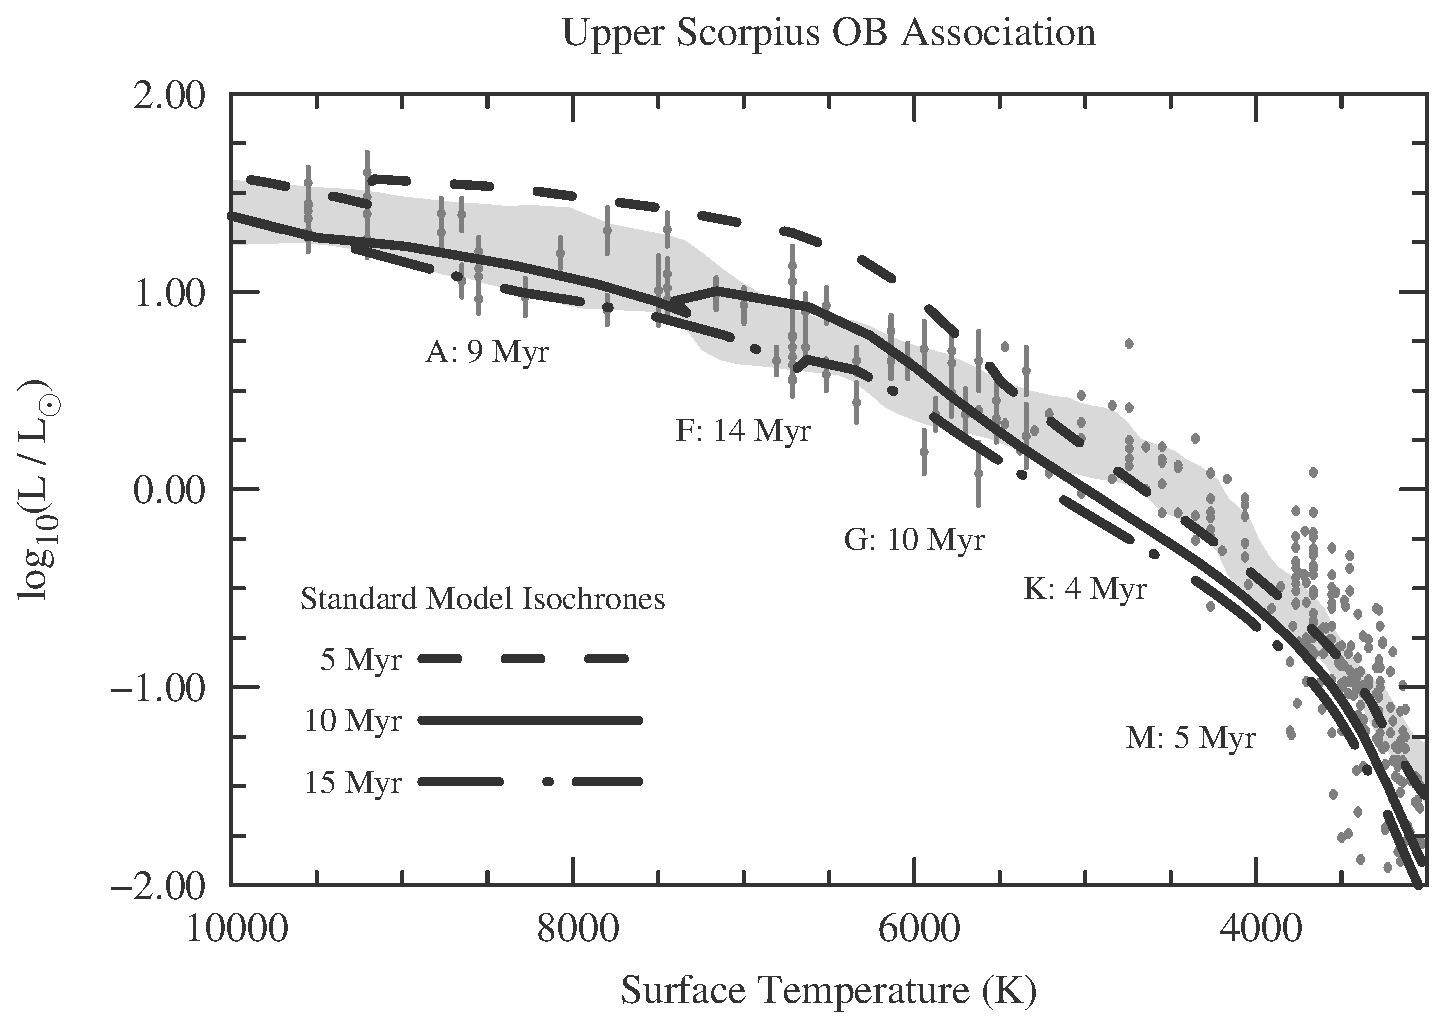
\includegraphics[width=0.65\columnwidth]{fig/USco_Age_Problems.eps}
	\caption{HR diagram for the Upper Scorpius OB Association. Stellar evolution model isochrones are shown in black. Labels show the ages inferred from different sub-populations in the association, highlighting a clear discordance between ages of hot and cool stars.}
	\label{fig:badhrd}
	\vspace{-0.2in}
\end{figure}

The difficulty is identifying which physics are missing from the models. Several mechanisms have been proposed to explain the luminosity spreads observed in HRDs of the youngest clusters. Examples include episodic accretion \citep{Baraffe2009, Baraffe2010} and starspots \citep{Somers2015b}, which can cause intrinsic variations in luminosity among a coeval population of stars. Until recently, there had not been a convincing demonstration of a physical mechanism to explain the observed effective-temperature-dependent ages or to explain the discrepancies between HRD and MRD age estimates. There had only been speculation that was focused on the usual suspects that are blamed for uncertainties in stellar models: convection, radiative opacities, or the absence of magnetic fields and starspots  \citep{Stassun2014, Soderblom2014, Herczeg2015}. 

% without supporting evidence


